\nwfilename{mainlitprog.nw}\nwbegindocs{0}\nwdocspar% ===> this file was generated automatically by noweave --- better not edit it

\section{Overall structure of \texttt{tspnng.py}}

The \texttt{tspnng.py} file at a high level divided into the following chunks, 
each of which is expanded upon in the coming sections. The \texttt{main.py} file used to run the \texttt{main()} function
from the command-line is more of a  scratchpad for testing the functions in this file, and later pointing the 
main to the appropriate test harnesses inside the \texttt{tspnng.py} file. Hence \texttt{main.py} will be developed 
independently of this document for convenience because it will be subject to continuous changes. .  

\nwenddocs{}\nwbegincode{1}\sublabel{NWaGG5Z-HXUTc-1}\nwmargintag{{\nwtagstyle{}\subpageref{NWaGG5Z-HXUTc-1}}}\moddef{tspnng.py~{\nwtagstyle{}\subpageref{NWaGG5Z-HXUTc-1}}}\endmoddef\nwstartdeflinemarkup\nwenddeflinemarkup

\LA{}Headers~{\nwtagstyle{}\subpageref{NWaGG5Z-2BmRoZ-1}}\RA{}
\LA{}Data Generation~{\nwtagstyle{}\subpageref{NWaGG5Z-2uhtAA-1}}\RA{}
\LA{}Generic utility classes and functions~{\nwtagstyle{}\subpageref{NWaGG5Z-4cZhfD-1}}\RA{}
\LA{}Functions for plotting and interacting~{\nwtagstyle{}\subpageref{NWaGG5Z-3DI44N-1}}\RA{}
\LA{}Functions for generating various graphs~{\nwtagstyle{}\subpageref{NWaGG5Z-2XNY09-1}}\RA{}
\LA{}Functions dealing with intersecting two geometric graphs~{\nwtagstyle{}\subpageref{NWaGG5Z-b3I3C-1}}\RA{}
\LA{}Testing hypotheses~{\nwtagstyle{}\subpageref{NWaGG5Z-3pWXcO-1}}\RA{}
\nwnotused{tspnng.py}\nwendcode{}\nwbegindocs{2}\nwdocspar


\nwenddocs{}\nwbegincode{3}\sublabel{NWaGG5Z-2BmRoZ-1}\nwmargintag{{\nwtagstyle{}\subpageref{NWaGG5Z-2BmRoZ-1}}}\moddef{Headers~{\nwtagstyle{}\subpageref{NWaGG5Z-2BmRoZ-1}}}\endmoddef\nwstartdeflinemarkup\nwusesondefline{\\{NWaGG5Z-HXUTc-1}}\nwprevnextdefs{\relax}{NWaGG5Z-2BmRoZ-2}\nwenddeflinemarkup
import matplotlib.pyplot as plt
import matplotlib as mpl
from matplotlib import rc
rc('font',**\{'family':'serif','serif':['Palatino']\})
rc('text', usetex=True)

import scipy as sp
import numpy as np
import random
import networkx as nx

from sklearn.cluster import KMeans
import argparse, os, sys, time
from colorama import init, Fore, Style, Back
init() # this line does nothing on Linux/Mac,
       # but is important for Windows to display
       # colored text. See https://pypi.org/project/colorama/
import yaml
\nwalsodefined{\\{NWaGG5Z-2BmRoZ-2}}\nwused{\\{NWaGG5Z-HXUTc-1}}\nwendcode{}\nwbegindocs{4}\nwdocspar


\section{Data Generation}

\nwenddocs{}\nwbegincode{5}\sublabel{NWaGG5Z-2uhtAA-1}\nwmargintag{{\nwtagstyle{}\subpageref{NWaGG5Z-2uhtAA-1}}}\moddef{Data Generation~{\nwtagstyle{}\subpageref{NWaGG5Z-2uhtAA-1}}}\endmoddef\nwstartdeflinemarkup\nwusesondefline{\\{NWaGG5Z-HXUTc-1}}\nwenddeflinemarkup
\LA{}TSPLIB data~{\nwtagstyle{}\subpageref{NWaGG5Z-Bg7qX-1}}\RA{}
\LA{}Synthetic data~{\nwtagstyle{}\subpageref{NWaGG5Z-1lO5Wy-1}}\RA{}
\nwused{\\{NWaGG5Z-HXUTc-1}}\nwendcode{}\nwbegindocs{6}\nwdocspar

\subsection{TSPLIB data-sets}

\autoref{fig:tsplib} is a screenshot of the entire opening page of \cite{reinelt1991tsplib}
that should more than suffice as an intro to this popular set of benchmarks for various TSP-like problems. \footnote{Prof. Sandor Fekete has a much larger collection of interesting TSP data-sets, I believe?}

\begin{figure}[htbp]
  \centering
  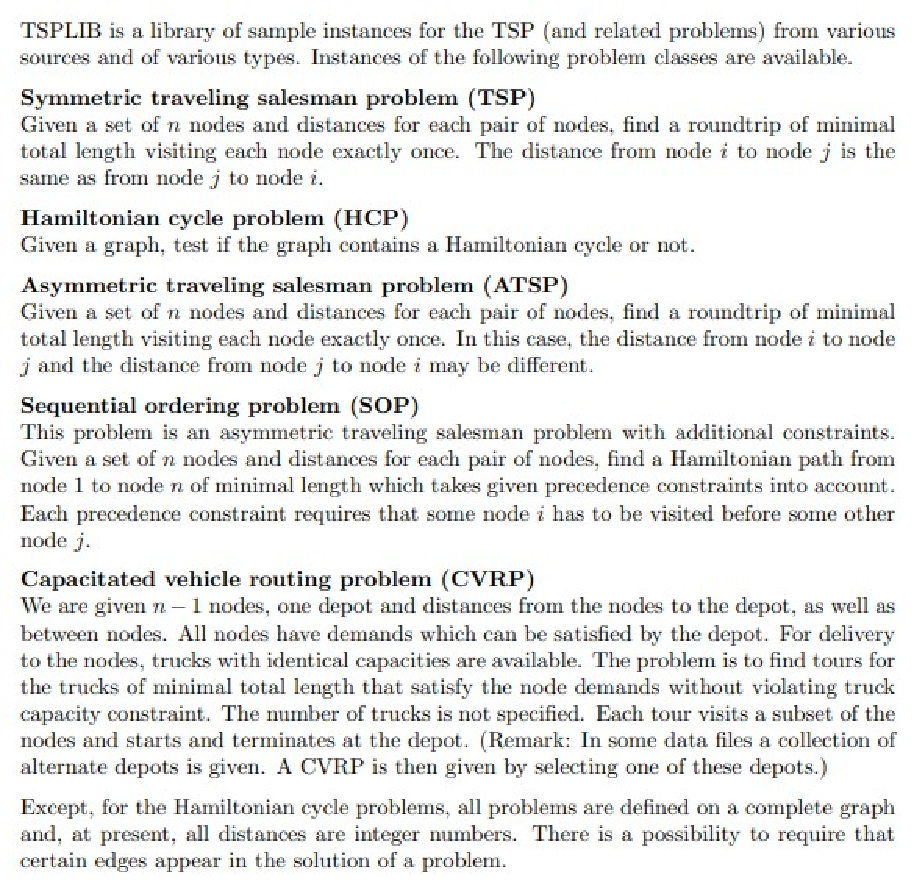
\includegraphics[width=9.4cm]{miscimages/tsplib-screenshot.pdf}
  \caption{\label{fig:tsplib} Screenshot of the opening page of \cite{reinelt1991tsplib} }
\end{figure}

In this document we will be interested in that subset of instances corresponding to the Symmetric TSP with the standard 
Euclidean Metric. Pages 9 through 11 of \cite{reinelt1991tsplib} contain 4-column tables with all Symmetric TSP instances. 
We will be focusing precisely on those instances which have their 3rd column marked ``\verb|EUC_2D|''.  

The entire symmetric TSP data-set has been downloaded into the 

\begin{displayquote}
\texttt{./sym-tsp-tsplib/instances/sym-tsp-tsplib/instances/tsplib\_symmetric\_tsp\_instances/} 
\end{displayquote}

directory. 
After writing a small Python script \footnote{\texttt{tsplib\_to\_yaml.py} in that same directory} the subset of \verb|EUC_2D| instances
were converted into the convenient YAML format and copied into the 

\begin{displayquote}
\color{blue}
\texttt{./sym-tsp-tsplib/instances/sym-tsp-tsplib/instances/euclidean\_instances\_yaml/} 
\end{displayquote}
directory. \textit{\textbf{Unless otherwise noted, we will retrict our attention to this directory when talking about TSPLIB data.}}

To see what the point-sets look like peep into the folder \verb|tsplib_euc2d_pictures_of_instances| contained in the top level directory of the code. 
Note that the numbers affixed to each instance name indicate the number of points in that instance. See \autoref{fig:tsplibinstances} for some examples. 

This chunk implements two functions: the first one returns the full path names of each of the Euclidean instances in an list and  the second one
reads in a TSPLIB instance (identified by its file-name e.g. \verb|'berlin52.yml'|) in the \verb|euclidean_instances_yaml| directory 
and returns a list of 2D points for that instance. 

\nwenddocs{}\nwbegincode{7}\sublabel{NWaGG5Z-Bg7qX-1}\nwmargintag{{\nwtagstyle{}\subpageref{NWaGG5Z-Bg7qX-1}}}\moddef{TSPLIB data~{\nwtagstyle{}\subpageref{NWaGG5Z-Bg7qX-1}}}\endmoddef\nwstartdeflinemarkup\nwusesondefline{\\{NWaGG5Z-2uhtAA-1}}\nwenddeflinemarkup

def get_names_of_all_euclidean2D_instances(dirpath=\\
         "./sym-tsp-tsplib/instances/euclidean_instances_yaml/" ):
     
     inst_names = []
     for name in os.listdir(dirpath):
         full_path = os.path.join(dirpath, name)
         if os.path.isfile(full_path):
             inst_names.append(name)
     return inst_names

def tsplib_instance_points(instance_file_name,\\
                           dirpath="./sym-tsp-tsplib/instances/euclidean_instances_yaml/"):

        print(Fore.GREEN+"Reading " + instance_file_name, Style.RESET_ALL)
        with open(dirpath+instance_file_name) as file:
            data = yaml.load(file, Loader=yaml.FullLoader)
            points = np.asarray(data['points'])
        
        return points 
           
\nwused{\\{NWaGG5Z-2uhtAA-1}}\nwendcode{}\nwbegindocs{8}\nwdocspar


 \begin{figure}[htbp]
   \centering
   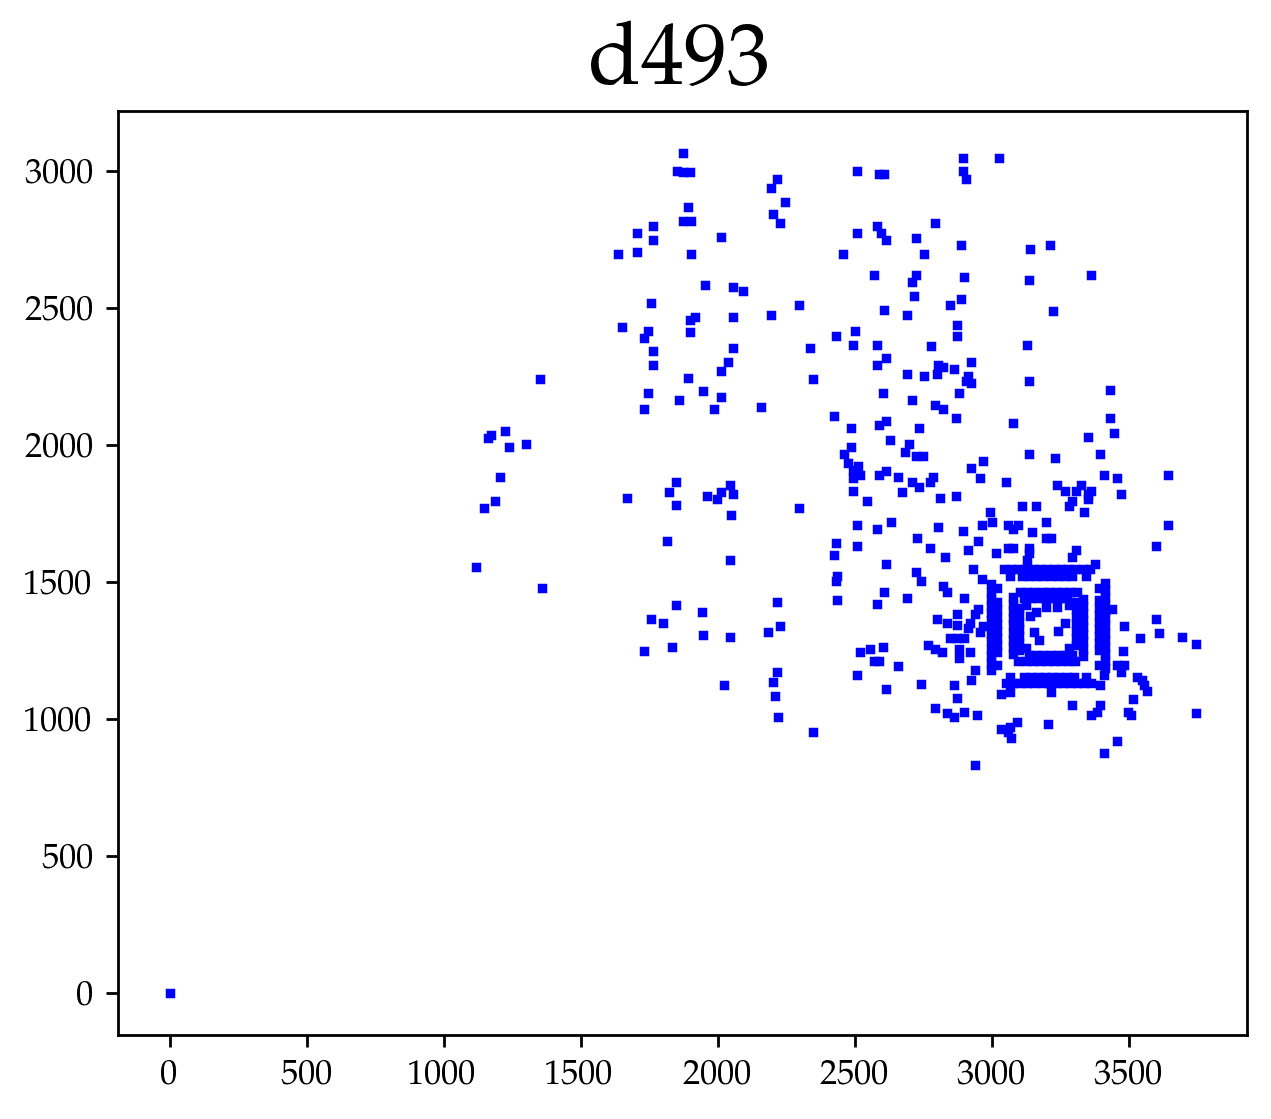
\includegraphics[width=7cm]{../tsplib_euc2d_pictures_of_instances/d493.png}
   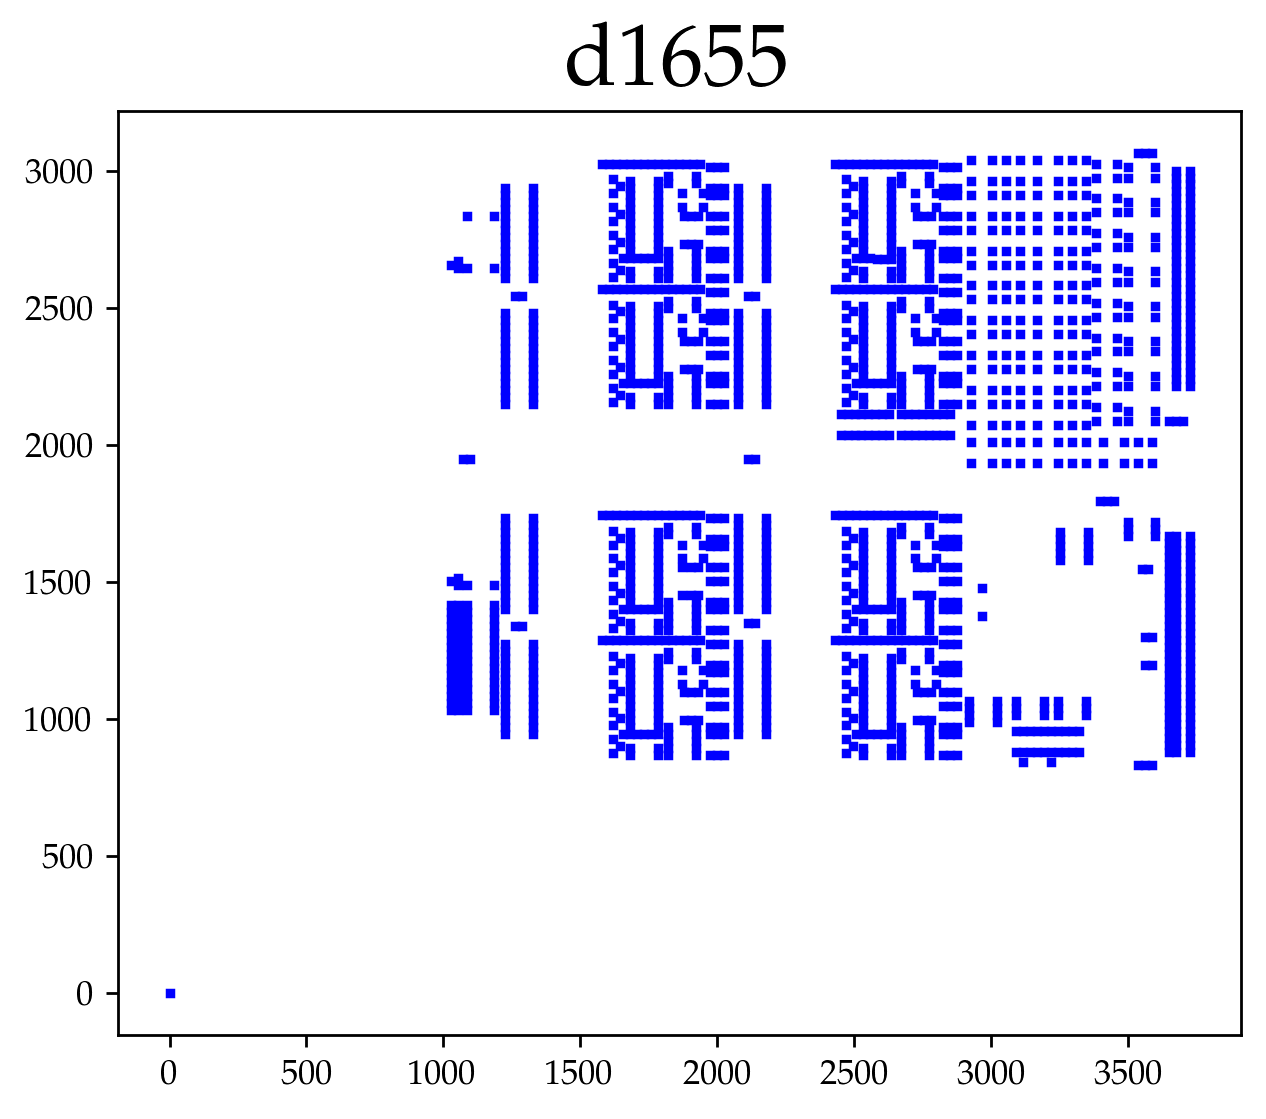
\includegraphics[width=7cm]{../tsplib_euc2d_pictures_of_instances/d1655.png}
   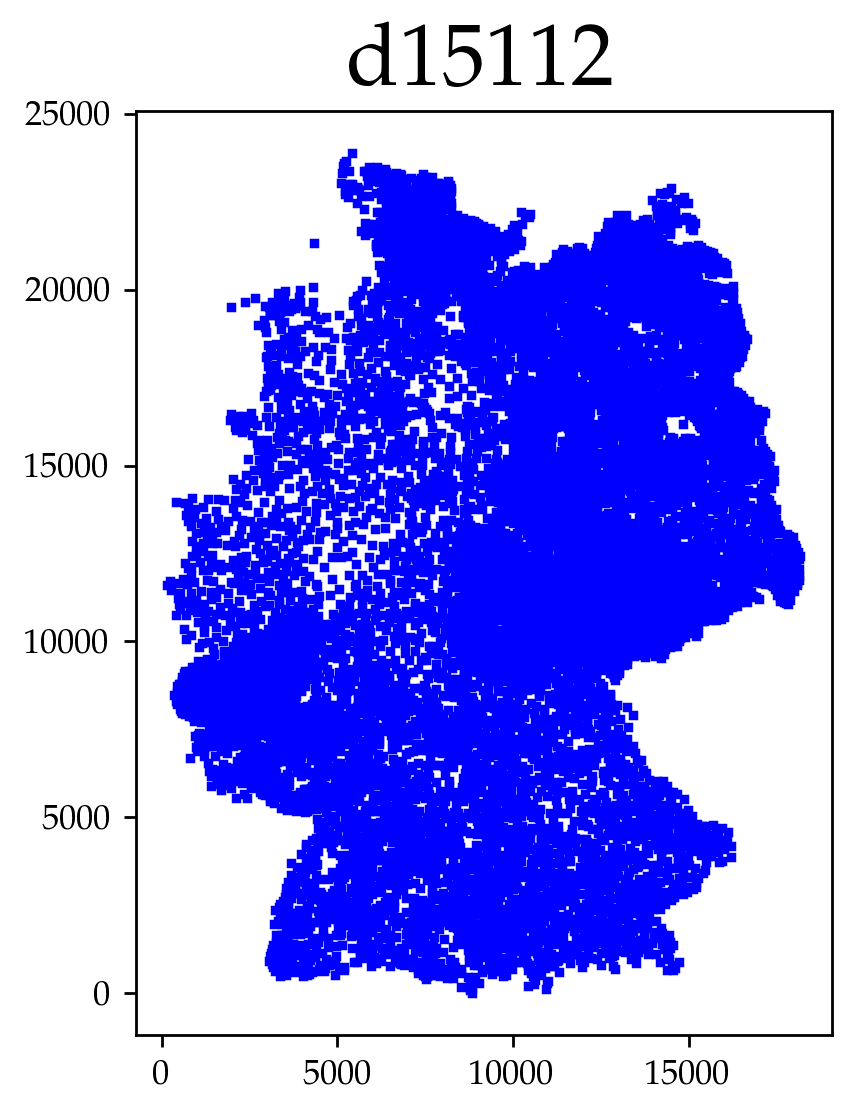
\includegraphics[width=5cm]{../tsplib_euc2d_pictures_of_instances/d15112.png}
   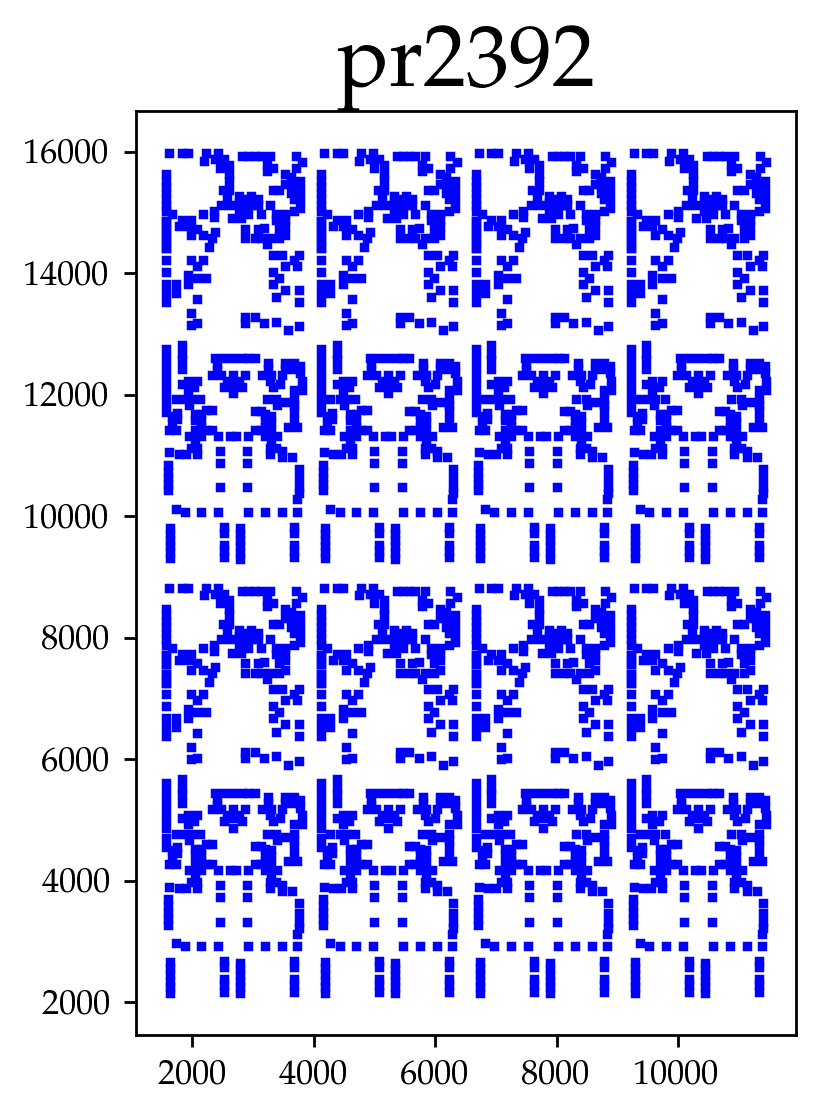
\includegraphics[width=6cm]{../tsplib_euc2d_pictures_of_instances/pr2392.png}
   \caption{\label{fig:tsplibinstances} Instances of four TSPLIB data sets for the Symmetric TSP with 2D Euclidean Metric}
 \end{figure}



\subsection{Synthetic data-sets}
Alongside TSPLIB we will also be using synthetic data-sets i.e. uniform and non-uniform point-sets generated inside the unit-square $[0,1] \times [0,1]$. 
Note that each point is represented as a numpy array of size 2. 

This chunk generates uniform and non-uniform point sets in $[0,1] \times [0,1]$. To generate non-uniform point-sets we basically 
take a small set of uniformly distributed random points in the square, place a small square centered around each such random point and then
generate the appropriate number of points uniformly inside each of those squares. \footnote{A somewhat similar method was used in Jon Bentley's experimental TSP paper}
The size of the square is proportional to the distance of the sampled point from the boundary of the unit square. Thus you will often see tight clusters
near the boundary as you increase the number of input points (\texttt{`numpts`}). This was done to make sure all points get generated in the unit square. 
This would make it convenient for the purposes of plotting. Other non-uniform point-generation schemes will later be considered depending on which 
direction our investigation proceeds. 


\nwenddocs{}\nwbegincode{9}\sublabel{NWaGG5Z-1lO5Wy-1}\nwmargintag{{\nwtagstyle{}\subpageref{NWaGG5Z-1lO5Wy-1}}}\moddef{Synthetic data~{\nwtagstyle{}\subpageref{NWaGG5Z-1lO5Wy-1}}}\endmoddef\nwstartdeflinemarkup\nwusesondefline{\\{NWaGG5Z-2uhtAA-1}}\nwenddeflinemarkup
def uniform_points(numpts):
     return  sp.rand(numpts, 2).tolist()

def non_uniform_points(numpts):

    cluster_size = int(np.sqrt(numpts)) 
    numcenters   = cluster_size
    centers      = sp.rand(numcenters,2).tolist()
    scale, points = 4.0, []

    for c in centers:
        cx, cy = c[0], c[1]
        sq_size      = min(cx,1-cx,cy, 1-cy)

        loc_pts_x    = np.random.uniform(low  = cx-sq_size/scale, 
                                         high = cx+sq_size/scale, 
                                         size = (cluster_size,))
        loc_pts_y    = np.random.uniform(low = cy-sq_size/scale, 
                                         high = cy+sq_size/scale, 
                                         size = (cluster_size,))

        points.extend(zip(loc_pts_x, loc_pts_y))

    num_remaining_pts = numpts - cluster_size * numcenters
    remaining_pts = sp.rand(num_remaining_pts, 2).tolist()
    points.extend(remaining_pts)
    return points
\nwused{\\{NWaGG5Z-2uhtAA-1}}\nwendcode{}\nwbegindocs{10}\nwdocspar

\section{Data Storage}
YAML\cite{ben2009yaml} is a convenient serialization and data-interchange format that we will be using 
for serializing output data of different experiments onto disk. Python has particularly good libraries for dealing with YAML. Basically, 
YAML records data in a format similar to a Python dictionary. Infact the \texttt{yaml} module provides a function that
transparently encodes any (appropriate) Python dictionary into a YAML file. In the function below, the 
\texttt{data} argument is a dictionary, and \texttt{dir\_name} and \texttt{file\_name} are strings. 
 
\nwenddocs{}\nwbegincode{11}\sublabel{NWaGG5Z-4cZhfD-1}\nwmargintag{{\nwtagstyle{}\subpageref{NWaGG5Z-4cZhfD-1}}}\moddef{Generic utility classes and functions~{\nwtagstyle{}\subpageref{NWaGG5Z-4cZhfD-1}}}\endmoddef\nwstartdeflinemarkup\nwusesondefline{\\{NWaGG5Z-HXUTc-1}}\nwprevnextdefs{\relax}{NWaGG5Z-4cZhfD-2}\nwenddeflinemarkup
def write_to_yaml_file(data, dir_name, file_name):
   with open(dir_name + '/' + file_name, 'w') as outfile:
          yaml.dump( data, outfile, default_flow_style = False)
\nwalsodefined{\\{NWaGG5Z-4cZhfD-2}}\nwused{\\{NWaGG5Z-HXUTc-1}}\nwendcode{}\nwbegindocs{12}\nwdocspar


\section{Setting up TSPNNGInput class}

The following class is used to keep track of the points inserted thus far, along with 
any other auxiliary information. It basically functions as a convenience wrapper class around 
the main input data (basically a bunch of points in $\RR^2$) and a wrapper function around 
various graph generators such as TSP, Delaunary, $k\text{-}$NNG etc. 

\nwenddocs{}\nwbegincode{13}\sublabel{NWaGG5Z-4cZhfD-2}\nwmargintag{{\nwtagstyle{}\subpageref{NWaGG5Z-4cZhfD-2}}}\moddef{Generic utility classes and functions~{\nwtagstyle{}\subpageref{NWaGG5Z-4cZhfD-1}}}\plusendmoddef\nwstartdeflinemarkup\nwusesondefline{\\{NWaGG5Z-HXUTc-1}}\nwprevnextdefs{NWaGG5Z-4cZhfD-1}{\relax}\nwenddeflinemarkup
class TSPNNGInput:
      def __init__(self, points=[]):
          self.points            = points

      def clearAllStates (self):
          self.points = []

      def generate_geometric_graph(self,graph_code):
           pass
\nwused{\\{NWaGG5Z-HXUTc-1}}\nwendcode{}\nwbegindocs{14}\nwdocspar

\section{Setting up the Interactive Canvas}
The following set of code blocks create an interactive matplotlib canvas onto which the user can insert points, and then 
run the appropriate algorithm to visualize the intersection of the TSP and various graphs. 

We first set up the run handler function (each ``run'' corresponds to a run of the code on a particular data-set generated synthetically)
by connecting the keyboard and mouse handlers to the canvas. 

\nwenddocs{}\nwbegincode{15}\sublabel{NWaGG5Z-3DI44N-1}\nwmargintag{{\nwtagstyle{}\subpageref{NWaGG5Z-3DI44N-1}}}\moddef{Functions for plotting and interacting~{\nwtagstyle{}\subpageref{NWaGG5Z-3DI44N-1}}}\endmoddef\nwstartdeflinemarkup\nwusesondefline{\\{NWaGG5Z-HXUTc-1}}\nwprevnextdefs{\relax}{NWaGG5Z-3DI44N-2}\nwenddeflinemarkup
def run_handler():
    fig, ax =  plt.subplots()
    run = TSPNNGInput()
    
    ax.set_xlim([xlim[0], xlim[1]])
    ax.set_ylim([ylim[0], ylim[1]])
    ax.set_aspect(1.0)
    ax.set_xticks([])
    ax.set_yticks([])
      
    mouseClick   = wrapperEnterRunPointsHandler(fig,ax, run)
    fig.canvas.mpl_connect('button_press_event' , mouseClick )
      
    keyPress     = wrapperkeyPressHandler(fig,ax, run)
    fig.canvas.mpl_connect('key_press_event', keyPress   )
    plt.show()
\nwalsodefined{\\{NWaGG5Z-3DI44N-2}\\{NWaGG5Z-3DI44N-3}\\{NWaGG5Z-3DI44N-4}\\{NWaGG5Z-3DI44N-5}}\nwused{\\{NWaGG5Z-HXUTc-1}}\nwendcode{}\nwbegindocs{16}\nwdocspar



There are two principal callback functions \verb|wrapperEnterRunPointshandler| and \verb|wrapperkeypresshandler| used in the code above. 
These encode the interaction between the mouse and keyboard to the matplotlib canvas. 

First we define the call back function for mouse-clicks. Double-clicking the left mouse button (denoted as ``button 1'' in the matplotlib world)
inserts a small circle patch representing a point. Note that each mouse click 
clears the canvas
and freshly draws the input point-set from scratch. 
This helps with modifying an existing input to check how solution changes. 

\nwenddocs{}\nwbegincode{17}\sublabel{NWaGG5Z-3DI44N-2}\nwmargintag{{\nwtagstyle{}\subpageref{NWaGG5Z-3DI44N-2}}}\moddef{Functions for plotting and interacting~{\nwtagstyle{}\subpageref{NWaGG5Z-3DI44N-1}}}\plusendmoddef\nwstartdeflinemarkup\nwusesondefline{\\{NWaGG5Z-HXUTc-1}}\nwprevnextdefs{NWaGG5Z-3DI44N-1}{NWaGG5Z-3DI44N-3}\nwenddeflinemarkup
xlim, ylim = [0,1], [0,1]
def wrapperEnterRunPointsHandler(fig, ax, run):
    def _enterPointsHandler(event):
        if event.name      == 'button_press_event'     and \\
           (event.button   == 1)                       and \\
            event.dblclick == True                     and \\
            event.xdata  != None                       and \\
            event.ydata  != None:

             newPoint = np.asarray([event.xdata, event.ydata])
             run.points.append( newPoint  )
             print("You inserted ", newPoint)

             patchSize  = (xlim[1]-xlim[0])/130.0
                   
             ax.clear()

             for pt in run.points:
                  ax.add_patch( mpl.patches.Circle( pt, radius = patchSize,
                                                    facecolor='blue', edgecolor='black'  ))

             ax.set_title('Points Inserted: ' + str(len(run.points)), \\
                           fontdict=\{'fontsize':25\})
             applyAxCorrection(ax)
             fig.canvas.draw()

    return _enterPointsHandler
\nwused{\\{NWaGG5Z-HXUTc-1}}\nwendcode{}\nwbegindocs{18}\nwdocspar

Now a call-back function for keyboard. Pressing \verb|`i'| or \verb|`I'| on the keyboard further prompts the 
user to insert a 2 or 3 letter code to indicate which graph should span the points. 

\nwenddocs{}\nwbegincode{19}\sublabel{NWaGG5Z-3DI44N-3}\nwmargintag{{\nwtagstyle{}\subpageref{NWaGG5Z-3DI44N-3}}}\moddef{Functions for plotting and interacting~{\nwtagstyle{}\subpageref{NWaGG5Z-3DI44N-1}}}\plusendmoddef\nwstartdeflinemarkup\nwusesondefline{\\{NWaGG5Z-HXUTc-1}}\nwprevnextdefs{NWaGG5Z-3DI44N-2}{NWaGG5Z-3DI44N-4}\nwenddeflinemarkup
def wrapperkeyPressHandler(fig,ax, run): 
       def _keyPressHandler(event):
               if event.key in ['n', 'N', 'u', 'U']: 
                     \LA{}Enter type of point set to generate~{\nwtagstyle{}\subpageref{NWaGG5Z-1TJD4t-1}}\RA{}                   
               elif event.key in ['t' or 'T']:
                     \LA{}Compute TSP and find common edges with various spanning graphs~{\nwtagstyle{}\subpageref{NWaGG5Z-1xEGS-1}}\RA{}
               elif event.key in ['i', 'I']:                     
                     \LA{}Compute spanning graph~{\nwtagstyle{}\subpageref{NWaGG5Z-33qwdb-1}}\RA{}    
               elif event.key in ['x', 'X']:
                     \LA{}Clear all line segments from the canvas~{\nwtagstyle{}\subpageref{NWaGG5Z-3ttuy9-1}}\RA{}
               elif event.key in ['c', 'C']: 
                     \LA{}Clear all states and the canvas~{\nwtagstyle{}\subpageref{NWaGG5Z-itHJV-1}}\RA{}
       return _keyPressHandler
\nwused{\\{NWaGG5Z-HXUTc-1}}\nwendcode{}\nwbegindocs{20}\nwdocspar

We now elaborate on the chunks in \verb|wrapperkeypresshandler|, and implement the boring technicalities. You 
can skip ahead to the next sections, at this point, if you wish. 

First we compute the TSP and then print a table mentioning how many of its edges are common to other
standard graphs. See \url{https://pypi.org/project/prettytable/} for more information on the 
prettytable module used to output data to terminal. 


\nwenddocs{}\nwbegincode{21}\sublabel{NWaGG5Z-2BmRoZ-2}\nwmargintag{{\nwtagstyle{}\subpageref{NWaGG5Z-2BmRoZ-2}}}\moddef{Headers~{\nwtagstyle{}\subpageref{NWaGG5Z-2BmRoZ-1}}}\plusendmoddef\nwstartdeflinemarkup\nwusesondefline{\\{NWaGG5Z-HXUTc-1}}\nwprevnextdefs{NWaGG5Z-2BmRoZ-1}{\relax}\nwenddeflinemarkup
from prettytable import PrettyTable
\nwused{\\{NWaGG5Z-HXUTc-1}}\nwendcode{}\nwbegindocs{22}\nwdocspar


\nwenddocs{}\nwbegincode{23}\sublabel{NWaGG5Z-1xEGS-1}\nwmargintag{{\nwtagstyle{}\subpageref{NWaGG5Z-1xEGS-1}}}\moddef{Compute TSP and find common edges with various spanning graphs~{\nwtagstyle{}\subpageref{NWaGG5Z-1xEGS-1}}}\endmoddef\nwstartdeflinemarkup\nwusesondefline{\\{NWaGG5Z-3DI44N-3}}\nwenddeflinemarkup
tsp_graph = get_concorde_tsp_graph(run.points)
graph_fns = [(get_delaunay_tri_graph, 'Delaunay Triangulation'), \\
             (get_mst_graph         , 'Minimum Spanning Tree'), \\
             (get_onion_graph       , 'Onion') ]

tbl             = PrettyTable()
tbl.field_names = ["Spanning Graph (G)", "G", "G \\cap T", "T", "(G \\cap T)/T"]

num_tsp_edges = len(tsp_graph.edges)
for ctr, (fn_body, fn_name) in zip(range(1,1+len(graph_fns)), graph_fns):
     geometric_graph = fn_body(run.points)
     num_graph_edges = len(geometric_graph.edges)
     common_edges    = list_common_edges(tsp_graph, geometric_graph)
     num_common_edges_with_tsp = len(common_edges)

     tbl.add_row([fn_name,                   \\
                num_graph_edges,           \\
                num_common_edges_with_tsp, \\
                num_tsp_edges,             \\
                "\{perc:3.2f\}".format(perc=1e2*num_common_edges_with_tsp/num_tsp_edges)+ ' %' ])
print(tbl)
render_graph(tsp_graph,fig,ax)
fig.canvas.draw()
\nwused{\\{NWaGG5Z-3DI44N-3}}\nwendcode{}\nwbegindocs{24}\nwdocspar

In a kind of ``dual'' demo, we now compute and render the various geometric graphs, and then mention how many 
edges each graph has in common with the TSP. Thus we can explore the intersection of the TSP with a graph
from the point-of-view of both the TSP and the graph. 

The user should type the code enclosed in the brackets (e.g. `\verb|dt|' for delaunay triangulation) to generate the 
indicated graph that spans the points. 

\nwenddocs{}\nwbegincode{25}\sublabel{NWaGG5Z-33qwdb-1}\nwmargintag{{\nwtagstyle{}\subpageref{NWaGG5Z-33qwdb-1}}}\moddef{Compute spanning graph~{\nwtagstyle{}\subpageref{NWaGG5Z-33qwdb-1}}}\endmoddef\nwstartdeflinemarkup\nwusesondefline{\\{NWaGG5Z-3DI44N-3}}\nwenddeflinemarkup
algo_str = input(Fore.YELLOW + "Enter code for the graph you need to span the points:\\n" + Style.RESET_ALL  +\\
                     "(knng)   k-Nearest Neighbor Graph        \\n"            +\\
                     "(mst)    Minimum Spanning Tree           \\n"            +\\
                     "(onion)  Onion                           \\n"            +\\
                     "(dt)     Delaunay Triangulation         \\n"             +\\
                     "(conc)   TSP computed by the Concorde TSP library \\n" +
                     "(pytsp)  TSP computed by the pure Python TSP library \\n")
algo_str = algo_str.lstrip()

if algo_str == 'knng':
      k_str = input('===> What value of k do you want? ')
      k     = int(k_str)
      geometric_graph = get_knng_graph(run.points,k)

elif algo_str == 'mst':
     geometric_graph = get_mst_graph(run.points)

elif algo_str == 'onion':
     geometric_graph = get_onion_graph(run.points)

elif algo_str == 'dt':
      geometric_graph = get_delaunay_tri_graph(run.points)

elif algo_str == 'conc':
     geometric_graph = get_concorde_tsp_graph(run.points)

elif algo_str == 'pytsp':
     geometric_graph = get_py_tsp_graph(run.points)

else:
      print(Fore.YELLOW, "I did not recognize that option.", Style.RESET_ALL)
      geometric_graph = None

common_edges = list_common_edges(get_concorde_tsp_graph(run.points), geometric_graph)
print("------------------------------------------------------------------------------")
print("Number of edges in " + algo_str + " graph (TOTAL)                          :", len(geometric_graph.edges))
print("Number of edges in " + algo_str + " graph which are also in Concorde TSP   :", len(common_edges))
print("------------------------------------------------------------------------------", Style.RESET_ALL)



ax.set_title("Graph Type: " + geometric_graph.graph['type'] + '\\n Number of nodes: ' + str(len(run.points)), fontdict=\{'fontsize':25\})
render_graph(geometric_graph,fig,ax)
fig.canvas.draw()
\nwused{\\{NWaGG5Z-3DI44N-3}}\nwendcode{}\nwbegindocs{26}\nwdocspar

If you want to enter a uniformly or non-uniformly distributed point-set in the unit-square press \verb|`u`| or \verb|`n`|
respectively after being prompted. 

\nwenddocs{}\nwbegincode{27}\sublabel{NWaGG5Z-1TJD4t-1}\nwmargintag{{\nwtagstyle{}\subpageref{NWaGG5Z-1TJD4t-1}}}\moddef{Enter type of point set to generate~{\nwtagstyle{}\subpageref{NWaGG5Z-1TJD4t-1}}}\endmoddef\nwstartdeflinemarkup\nwusesondefline{\\{NWaGG5Z-3DI44N-3}}\nwenddeflinemarkup
numpts = int(input("\\nHow many points should I generate?: ")) 
run.clearAllStates()
ax.cla()
applyAxCorrection(ax)

ax.set_xticks([])
ax.set_yticks([])
fig.texts = []
                 
if event.key in ['n', 'N']: 
        run.points = non_uniform_points(numpts)
else : 
        run.points = uniform_points(numpts)

patchSize  = (xlim[1]-xlim[0])/140.0

for site in run.points:      
    ax.add_patch(mpl.patches.Circle(site, radius = patchSize, \\
                 facecolor='blue',edgecolor='black' ))

ax.set_title('Points generated: ' + str(len(run.points)), fontdict=\{'fontsize':25\})
fig.canvas.draw()
\nwused{\\{NWaGG5Z-3DI44N-3}}\nwendcode{}\nwbegindocs{28}\nwdocspar



Sometimes, you just want to clear the edges of the network from the graph, so that
a new graph can be rendered in its place on the points. For that, you need to press
`x` or `X`. 

\nwenddocs{}\nwbegincode{29}\sublabel{NWaGG5Z-3ttuy9-1}\nwmargintag{{\nwtagstyle{}\subpageref{NWaGG5Z-3ttuy9-1}}}\moddef{Clear all line segments from the canvas~{\nwtagstyle{}\subpageref{NWaGG5Z-3ttuy9-1}}}\endmoddef\nwstartdeflinemarkup\nwusesondefline{\\{NWaGG5Z-3DI44N-3}}\nwenddeflinemarkup
print(Fore.GREEN, 'Removing network edges from canvas' ,Style.RESET_ALL)
ax.lines=[]
applyAxCorrection(ax)
fig.canvas.draw()
\nwused{\\{NWaGG5Z-3DI44N-3}}\nwendcode{}\nwbegindocs{30}\nwdocspar

If you want to wipe the canvas and the point-cloud data (and everything else \ldots) clean, 
then press \verb|`c`|. 

\nwenddocs{}\nwbegincode{31}\sublabel{NWaGG5Z-itHJV-1}\nwmargintag{{\nwtagstyle{}\subpageref{NWaGG5Z-itHJV-1}}}\moddef{Clear all states and the canvas~{\nwtagstyle{}\subpageref{NWaGG5Z-itHJV-1}}}\endmoddef\nwstartdeflinemarkup\nwusesondefline{\\{NWaGG5Z-3DI44N-3}}\nwenddeflinemarkup
run.clearAllStates()
ax.cla()
                                 
applyAxCorrection(ax)
ax.set_xticks([])
ax.set_yticks([])
                                    
fig.texts = []
fig.canvas.draw()
\nwused{\\{NWaGG5Z-3DI44N-3}}\nwendcode{}\nwbegindocs{32}\nwdocspar





Often the \verb|ax| object has to be reset and cleaned of the various segment and circle patches, or even resetting the 
aspect ratio of the \verb|ax| object to be 1.0. These ``cleanup'' functions that were called in some of the code blocks above 
are implemented next. 

\nwenddocs{}\nwbegincode{33}\sublabel{NWaGG5Z-3DI44N-4}\nwmargintag{{\nwtagstyle{}\subpageref{NWaGG5Z-3DI44N-4}}}\moddef{Functions for plotting and interacting~{\nwtagstyle{}\subpageref{NWaGG5Z-3DI44N-1}}}\plusendmoddef\nwstartdeflinemarkup\nwusesondefline{\\{NWaGG5Z-HXUTc-1}}\nwprevnextdefs{NWaGG5Z-3DI44N-3}{NWaGG5Z-3DI44N-5}\nwenddeflinemarkup
def applyAxCorrection(ax):
      ax.set_xlim([xlim[0], xlim[1]])
      ax.set_ylim([ylim[0], ylim[1]])
      ax.set_aspect(1.0)

def clearPatches(ax):
    for index , patch in zip(range(len(ax.patches)), ax.patches):
        if isinstance(patch, mpl.patches.Polygon) == True:
            patch.remove()
    ax.lines[:]=[]
    applyAxCorrection(ax)

def clearAxPolygonPatches(ax):

    for index , patch in zip(range(len(ax.patches)), ax.patches):
        if isinstance(patch, mpl.patches.Polygon) == True:
            patch.remove()
    ax.lines[:]=[]
    applyAxCorrection(ax)
\nwused{\\{NWaGG5Z-HXUTc-1}}\nwendcode{}\nwbegindocs{34}\nwdocspar


\section{Generating various geometric graphs}

For manipulating abstract graphs we use the NetworkX \cite{hagberg2008exploring} \footnote{already available inside the Anaconda Python distribution by default}. 
This section deals with generating the various geometric graphs using packages like Scipy and Sklearn and then converting them into a NetworkX graph
with the necessary edge and node attributes. Note that all the nodes in the abstract constructed below have the same numbering across all grap have the same 
numbering across all graphs: namely, the order in which the points occur in the \verb|points| array argument. 


\subsection{$k\text{-}$NNG}

\definecolor{bisque}{rgb}{1.0, 0.89, 0.77}
\renewcommand\fbox{\fcolorbox{bisque}{white}}
\setlength\fboxrule{0.1pt}

\begin{figure}[ht]
  \centering
  \fbox{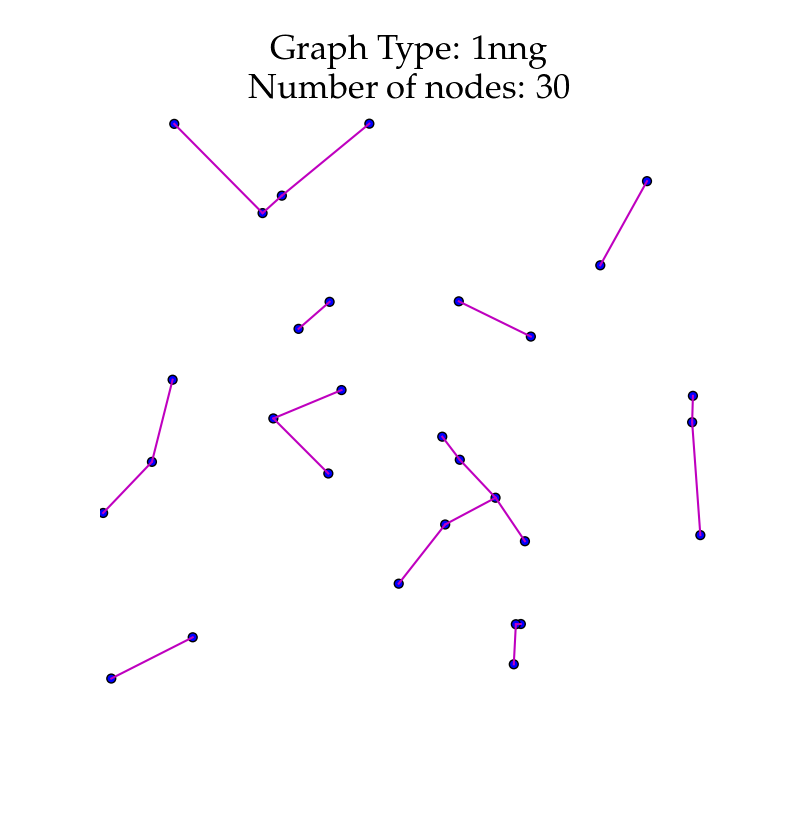
\includegraphics[width=5cm]{./miscimages/1nng-example.png}} \hfill
  \fbox{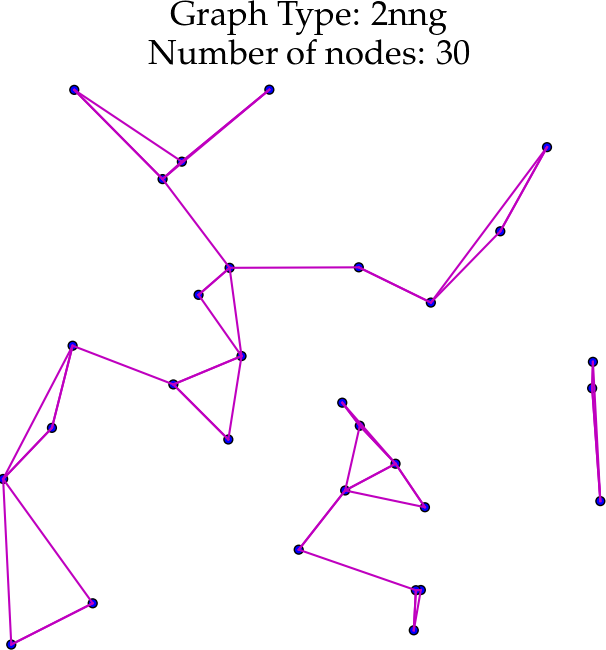
\includegraphics[width=5cm]{./miscimages/2nng-example.png}} \hfill
  \fbox{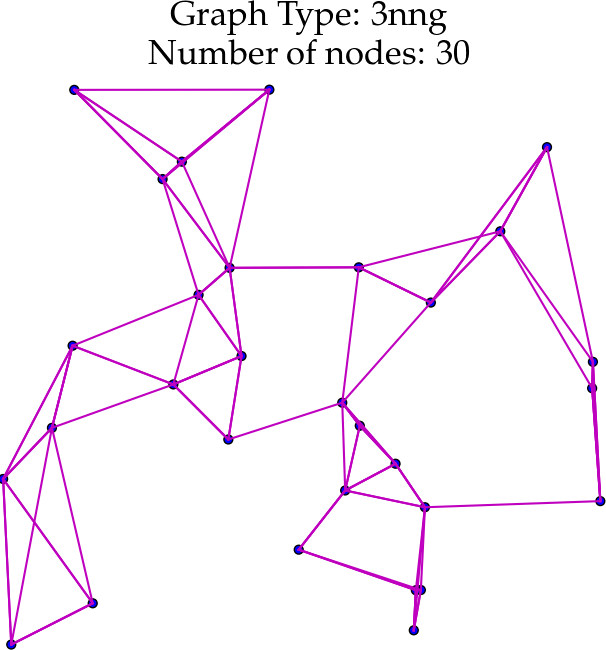
\includegraphics[width=5cm]{./miscimages/3nng-example.png}}
  \caption{\label{fig:knng} Generating the $k$-NNG graphs with Scikit-Learn for various value of $k$ on the same set of 30 randomly generated points. Note that we are considering these graphs as undirected.}
\end{figure}


We use the nearest neighbor routine from the Scikit-learn \cite{pedregosa2011scikit} library. The documentation
for the various nearest neighor methods implemented therein can be found at 
\url{https://bit.ly/3nTQkqV}. Note that for the nearest-neighbor function of sklearn the $k\text{-}$ nearest-neighbors of a point
includes the point itself. Thus we use $(k+1)$ in the argument to the \verb|NearestNeighbors| function below, and take the last $k$
elements in the list returned --- the neighbors of a point are reported by that function in increasing order of distance from that point. 

\nwenddocs{}\nwbegincode{35}\sublabel{NWaGG5Z-2XNY09-1}\nwmargintag{{\nwtagstyle{}\subpageref{NWaGG5Z-2XNY09-1}}}\moddef{Functions for generating various graphs~{\nwtagstyle{}\subpageref{NWaGG5Z-2XNY09-1}}}\endmoddef\nwstartdeflinemarkup\nwusesondefline{\\{NWaGG5Z-HXUTc-1}}\nwprevnextdefs{\relax}{NWaGG5Z-2XNY09-2}\nwenddeflinemarkup
def get_knng_graph(points,k):
     from sklearn.neighbors import NearestNeighbors
     points     = np.array(points)
     coords     = [\{"coods":pt\} for pt in points]
     knng_graph = nx.Graph()
     knng_graph.add_nodes_from(zip(range(len(points)), coords))
     nbrs = NearestNeighbors(n_neighbors=(k+1), algorithm='ball_tree').fit(points)
     distances, indices = nbrs.kneighbors(points)
     edge_list = []

     for nbidxs in indices:
          nfix = nbidxs[0]
          edge_list.extend([(nfix,nvar) for nvar in nbidxs[1:]])

     knng_graph.add_edges_from(  edge_list  )
     knng_graph.graph['type']   = str(k)+'nng'
     knng_graph.graph['weight'] =  None # TODO, also edge weights for each edge!!!
     return knng_graph
\nwalsodefined{\\{NWaGG5Z-2XNY09-2}\\{NWaGG5Z-2XNY09-3}\\{NWaGG5Z-2XNY09-4}\\{NWaGG5Z-2XNY09-5}\\{NWaGG5Z-2XNY09-6}}\nwused{\\{NWaGG5Z-HXUTc-1}}\nwendcode{}\nwbegindocs{36}\nwdocspar


\subsection{Delaunay Triangulation}

\begin{figure}[ht]
  \centering
  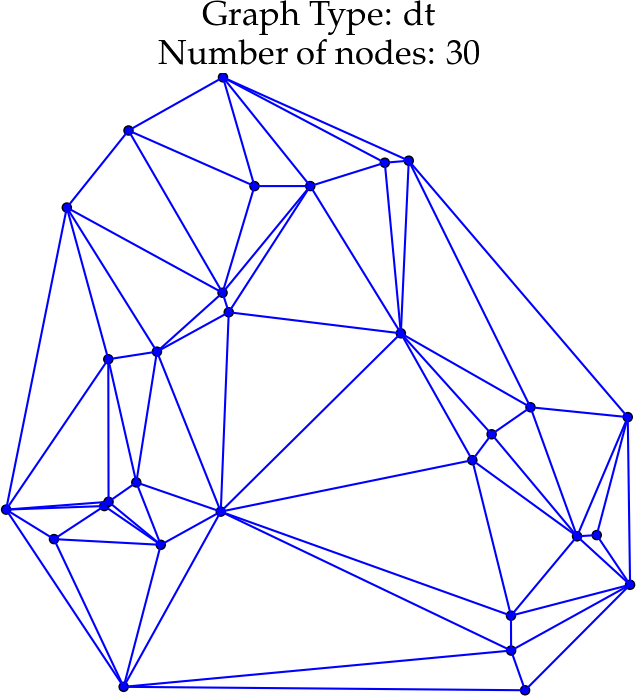
\includegraphics[width=7cm]{./miscimages/dt-example.png}
  \caption{\label{fig:dt} Example of a Delaunay Triangulation computed by SciPy on 30 randomly generated points}
\end{figure}


We use the  \href{https://docs.scipy.org/doc/scipy/reference/generated/scipy.spatial.Delaunay.html}{blackbox routine} 
for computing this graph implmeneted in Scipy \cite{virtanen2020scipy}. 

\nwenddocs{}\nwbegincode{37}\sublabel{NWaGG5Z-2XNY09-2}\nwmargintag{{\nwtagstyle{}\subpageref{NWaGG5Z-2XNY09-2}}}\moddef{Functions for generating various graphs~{\nwtagstyle{}\subpageref{NWaGG5Z-2XNY09-1}}}\plusendmoddef\nwstartdeflinemarkup\nwusesondefline{\\{NWaGG5Z-HXUTc-1}}\nwprevnextdefs{NWaGG5Z-2XNY09-1}{NWaGG5Z-2XNY09-3}\nwenddeflinemarkup
def get_delaunay_tri_graph(points):
     from scipy.spatial import Delaunay
     points       = np.array(points)
     coords       = [\{"coods":pt\} for pt in points]
     tri          = Delaunay(points)
     deltri_graph = nx.Graph()

     deltri_graph.add_nodes_from(zip(range(len(points)), coords))

     edge_list = []
     for (i,j,k) in tri.simplices:
         edge_list.extend([(i,j),(j,k),(k,i)])    
     deltri_graph.add_edges_from(  edge_list  )
     
     total_weight_of_edges = 0.0
     for edge in deltri_graph.edges:
           n1, n2 = edge
           pt1 = deltri_graph.nodes[n1]['coods'] 
           pt2 = deltri_graph.nodes[n2]['coods']
           edge_wt = np.linalg.norm(pt1-pt2)

           deltri_graph.edges[n1,n2]['weight'] = edge_wt
           total_weight_of_edges = total_weight_of_edges + edge_wt 
     
     deltri_graph.graph['weight'] = total_weight_of_edges
     deltri_graph.graph['type']   = 'dt'

     return deltri_graph
\nwused{\\{NWaGG5Z-HXUTc-1}}\nwendcode{}\nwbegindocs{38}\nwdocspar


\subsection{Minimum Spanning Tree}

\begin{figure}[ht]
  \centering
  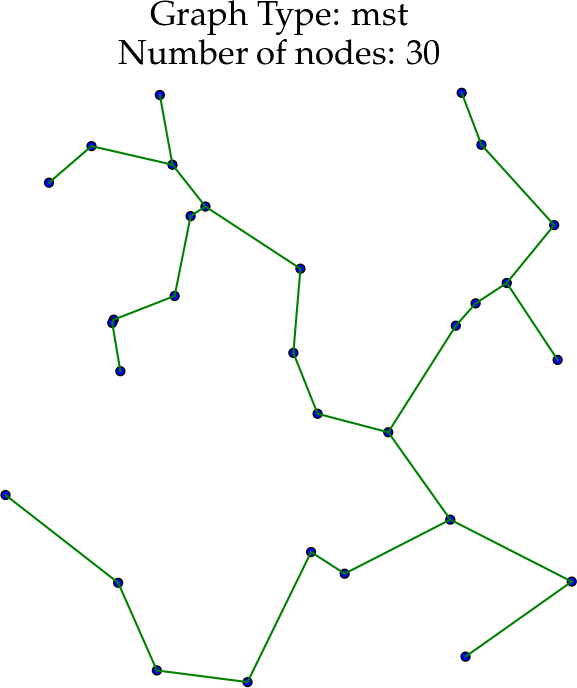
\includegraphics[width=6cm]{./miscimages/mst-example.png}
  \caption{\label{fig:mst} Example of a Minimum Spanning Tree computed by NetworkX on 30 randomly generated points}
\end{figure}


From elementary CG, we know that the MST of a set of points in the plane is a subset of the delaunay triangulation. Thus to compute the MST,
it suffices to compute the MST of the corresponding delaunay triangulation. 
See \href{https://networkx.github.io/documentation/stable/reference/algorithms/generated/networkx.algorithms.tree.mst.minimum_spanning_edges.html}{this page}
for a documentation of the code in NetworkX used to compute the MST on an abstract weighted undirected graph. Note that along with the Kruskal method (used below), both Prim's and Boruvka's 
algorithms have also been implemented in that library. 

\nwenddocs{}\nwbegincode{39}\sublabel{NWaGG5Z-2XNY09-3}\nwmargintag{{\nwtagstyle{}\subpageref{NWaGG5Z-2XNY09-3}}}\moddef{Functions for generating various graphs~{\nwtagstyle{}\subpageref{NWaGG5Z-2XNY09-1}}}\plusendmoddef\nwstartdeflinemarkup\nwusesondefline{\\{NWaGG5Z-HXUTc-1}}\nwprevnextdefs{NWaGG5Z-2XNY09-2}{NWaGG5Z-2XNY09-4}\nwenddeflinemarkup

def get_mst_graph(points):

     points = np.array(points)
     deltri_graph = get_delaunay_tri_graph(points)
     mst_graph = nx.algorithms.tree.mst.minimum_spanning_tree(deltri_graph, \\
                                                              algorithm='kruskal')
     mst_graph.graph['type']   = 'mst'
     return mst_graph
\nwused{\\{NWaGG5Z-HXUTc-1}}\nwendcode{}\nwbegindocs{40}\nwdocspar


\subsection{The Onion}

\begin{figure}[H]
  \centering
  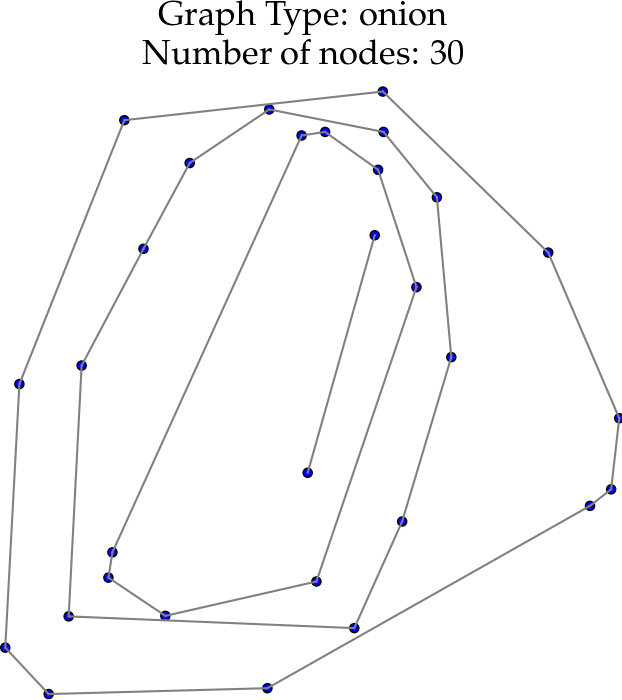
\includegraphics[width=6cm]{./miscimages/onion-example.png}
  \caption{\label{fig:onion} Example of the Onion graph computed with computed with QHull (through SciPy) on 30 randomly generated points }
\end{figure}



Here we compute successive convex-hull of the point-set: compute the convex hull of the points, delete the hull points, 
compute the convex hull of this smaller point-set, repeating this process till we run out of points. 

The resulting sequence of convex layers form a graph called the onion. 

\nwenddocs{}\nwbegincode{41}\sublabel{NWaGG5Z-2XNY09-4}\nwmargintag{{\nwtagstyle{}\subpageref{NWaGG5Z-2XNY09-4}}}\moddef{Functions for generating various graphs~{\nwtagstyle{}\subpageref{NWaGG5Z-2XNY09-1}}}\plusendmoddef\nwstartdeflinemarkup\nwusesondefline{\\{NWaGG5Z-HXUTc-1}}\nwprevnextdefs{NWaGG5Z-2XNY09-3}{NWaGG5Z-2XNY09-5}\nwenddeflinemarkup

def get_onion_graph(points):
     from scipy.spatial import ConvexHull
     points      = np.asarray(points)     
     points_tmp  = points.copy()
     numpts      = len(points)
     onion_graph = nx.Graph()
     numpts_proc = -1

     \LA{} Definition of \verb|circular_edge_zip|~{\nwtagstyle{}\subpageref{NWaGG5Z-2QHw3A-1}}\RA{}
     while len(points_tmp) >= 3:
           \LA{}Generate convex hull of points remaining in \verb|points_tmp|~{\nwtagstyle{}\subpageref{NWaGG5Z-1qB5IG-1}}\RA{}
           \LA{}Update \verb|onion_graph|~{\nwtagstyle{}\subpageref{NWaGG5Z-24g2s3-1}}\RA{}
           \LA{}Remove points reported in the convex hull from \verb|points_tmp|~{\nwtagstyle{}\subpageref{NWaGG5Z-ArYW6-1}}\RA{}

     if len(points_tmp) == 2:
          \LA{}Join two remaining points by an edge in \verb|onion_graph|~{\nwtagstyle{}\subpageref{NWaGG5Z-1QE0qW-1}}\RA{}
     elif len(points_tmp) == 1:
          \LA{}Add the remaining points as a node in \verb|onion_graph|~{\nwtagstyle{}\subpageref{NWaGG5Z-2GN3bQ-1}}\RA{}
 
     onion_graph.graph['type'] = 'onion'
     return onion_graph
\nwused{\\{NWaGG5Z-HXUTc-1}}\nwendcode{}\nwbegindocs{42}\nwdocspar


Note that the convex hull is computed by Scipy using the Qhull library as mentioned in the \href{https://docs.scipy.org/doc/scipy/reference/generated/scipy.spatial.ConvexHull.html}{docs}. 
\nwenddocs{}\nwbegincode{43}\sublabel{NWaGG5Z-1qB5IG-1}\nwmargintag{{\nwtagstyle{}\subpageref{NWaGG5Z-1qB5IG-1}}}\moddef{Generate convex hull of points remaining in \verb|points_tmp|~{\nwtagstyle{}\subpageref{NWaGG5Z-1qB5IG-1}}}\endmoddef\nwstartdeflinemarkup\nwusesondefline{\\{NWaGG5Z-2XNY09-4}}\nwenddeflinemarkup
hull            = ConvexHull(points_tmp)
pts_on_hull     = [points_tmp[i] for i in hull.vertices]
coords          = [\{"coods":pt\} for pt in pts_on_hull]
\nwused{\\{NWaGG5Z-2XNY09-4}}\nwendcode{}\nwbegindocs{44}\nwdocspar


\nwenddocs{}\nwbegincode{45}\sublabel{NWaGG5Z-24g2s3-1}\nwmargintag{{\nwtagstyle{}\subpageref{NWaGG5Z-24g2s3-1}}}\moddef{Update \verb|onion_graph|~{\nwtagstyle{}\subpageref{NWaGG5Z-24g2s3-1}}}\endmoddef\nwstartdeflinemarkup\nwusesondefline{\\{NWaGG5Z-2XNY09-4}}\nwenddeflinemarkup
new_node_idxs   = range(numpts_proc+1, numpts_proc+len(hull.vertices)+1)
onion_graph.add_nodes_from(zip(new_node_idxs, coords))
onion_graph.add_edges_from(circular_edge_zip(new_node_idxs))
\nwused{\\{NWaGG5Z-2XNY09-4}}\nwendcode{}\nwbegindocs{46}\nwdocspar


Given a set of node ids of a graph provided as a list of 
integers, the following function, returns a cycle of edges with successive nodes joined in
the order provided. e.g. $[1,2,3] \rarr [(1,2),(2,3),(3,1)]$. Convenient to have this defined 
separately. 

\nwenddocs{}\nwbegincode{47}\sublabel{NWaGG5Z-2QHw3A-1}\nwmargintag{{\nwtagstyle{}\subpageref{NWaGG5Z-2QHw3A-1}}}\moddef{ Definition of \verb|circular_edge_zip|~{\nwtagstyle{}\subpageref{NWaGG5Z-2QHw3A-1}}}\endmoddef\nwstartdeflinemarkup\nwusesondefline{\\{NWaGG5Z-2XNY09-4}}\nwenddeflinemarkup
def circular_edge_zip(xs):
    xs = list(xs) # in the event that xs is of the zip or range type 
    if len(xs) in [0,1] :
         zipl = []
    elif len(xs) == 2 :
         zipl = [(xs[0],xs[1])]
    else:
         zipl = list(zip(xs,xs[1:]+xs[:1]))
    return zipl

\nwused{\\{NWaGG5Z-2XNY09-4}}\nwendcode{}\nwbegindocs{48}\nwdocspar




\nwenddocs{}\nwbegincode{49}\sublabel{NWaGG5Z-ArYW6-1}\nwmargintag{{\nwtagstyle{}\subpageref{NWaGG5Z-ArYW6-1}}}\moddef{Remove points reported in the convex hull from \verb|points_tmp|~{\nwtagstyle{}\subpageref{NWaGG5Z-ArYW6-1}}}\endmoddef\nwstartdeflinemarkup\nwusesondefline{\\{NWaGG5Z-2XNY09-4}}\nwenddeflinemarkup
numpts_proc  = numpts_proc + len(hull.vertices)
rem_pts_idxs = list(set(range(len(points_tmp)))-set(hull.vertices)) 
points_tmp   = [ points_tmp[idx] for idx in rem_pts_idxs ]
coords       = [\{"coods":pt\} for pt in points]
\nwused{\\{NWaGG5Z-2XNY09-4}}\nwendcode{}\nwbegindocs{50}\nwdocspar


There are two edge cases: when only two points and one point remain. These cases, cannot be handled by Qhull (It reports an error at the terminal,
saying it needs at least three points must be provided as input). Hence the separate treatment in the following two chunks. 


When two nodes, remain, we just join them by an edge. 

\nwenddocs{}\nwbegincode{51}\sublabel{NWaGG5Z-1QE0qW-1}\nwmargintag{{\nwtagstyle{}\subpageref{NWaGG5Z-1QE0qW-1}}}\moddef{Join two remaining points by an edge in \verb|onion_graph|~{\nwtagstyle{}\subpageref{NWaGG5Z-1QE0qW-1}}}\endmoddef\nwstartdeflinemarkup\nwusesondefline{\\{NWaGG5Z-2XNY09-4}}\nwenddeflinemarkup
p, l = numpts_proc+1, numpts_proc+2
onion_graph.add_node(p)
onion_graph.add_node(l)
onion_graph.nodes[p]['coods'] = points_tmp[0]
onion_graph.nodes[l]['coods'] = points_tmp[1]
onion_graph.add_edge(p,l)
\nwused{\\{NWaGG5Z-2XNY09-4}}\nwendcode{}\nwbegindocs{52}\nwdocspar

No edges to add here, just the node. 

\nwenddocs{}\nwbegincode{53}\sublabel{NWaGG5Z-2GN3bQ-1}\nwmargintag{{\nwtagstyle{}\subpageref{NWaGG5Z-2GN3bQ-1}}}\moddef{Add the remaining points as a node in \verb|onion_graph|~{\nwtagstyle{}\subpageref{NWaGG5Z-2GN3bQ-1}}}\endmoddef\nwstartdeflinemarkup\nwusesondefline{\\{NWaGG5Z-2XNY09-4}}\nwenddeflinemarkup
l = numpts_proc+1 
onion_graph.add_node(l)
onion_graph.nodes[l]['cood'] = points_tmp[0]
\nwused{\\{NWaGG5Z-2XNY09-4}}\nwendcode{}\nwbegindocs{54}\nwdocspar




\subsection{Traveling Saleman Tour (Cycle)}

\begin{figure}[ht]
  \centering
  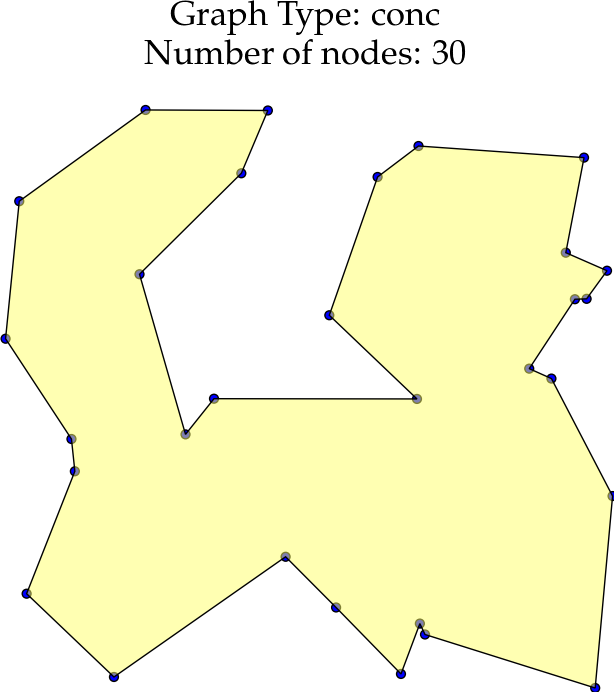
\includegraphics[width=6cm]{./miscimages/conc-example.png}
  \caption{\label{fig:tsp} Example of an \underline{optimal} TSP tour computed with Concorde  on 30 randomly generated points }
\end{figure}


We use two separate independent routines that each compute the TSP. One is the 
\verb|tsp| module available at \link{https://pypi.org/project/tsp/}
the other being, Concorde, through its Python interface (whose github page can be accessed at 
\link{https://github.com/jvkersch/pyconcorde}. Anedoctally speaking the first solver works relatively 
quickly on point-sets upto size 30. Because of its simplicity, we used it in the intial stages of writing
this report. It is clearly not competitive with Concorde (which can solve a 300 size instances in a couple of seconds), 
but it serves as a useful backup routine, in the event that a machine faces problems with the installation of PyConcorde.

\subsubsection{* Using the \texttt{tsp} library}
\nwenddocs{}\nwbegincode{55}\sublabel{NWaGG5Z-2XNY09-5}\nwmargintag{{\nwtagstyle{}\subpageref{NWaGG5Z-2XNY09-5}}}\moddef{Functions for generating various graphs~{\nwtagstyle{}\subpageref{NWaGG5Z-2XNY09-1}}}\plusendmoddef\nwstartdeflinemarkup\nwusesondefline{\\{NWaGG5Z-HXUTc-1}}\nwprevnextdefs{NWaGG5Z-2XNY09-4}{NWaGG5Z-2XNY09-6}\nwenddeflinemarkup
def get_py_tsp_graph(points):
     import tsp
     points = np.array(points)
     coords = [\{"coods":pt\} for pt in points]
     \LA{}Generate TSP cycle and convert into NetworkX graph~{\nwtagstyle{}\subpageref{NWaGG5Z-ixiQd-1}}\RA{}
     \LA{}Compute weight of each edge and total edge weight~{\nwtagstyle{}\subpageref{NWaGG5Z-3homP2-1}}\RA{}
     \LA{}Set graph attributes~{\nwtagstyle{}\subpageref{NWaGG5Z-1NBtrs-1}}\RA{}     
     return tsp_graph
\nwused{\\{NWaGG5Z-HXUTc-1}}\nwendcode{}\nwbegindocs{56}\nwdocspar


\nwenddocs{}\nwbegincode{57}\sublabel{NWaGG5Z-ixiQd-1}\nwmargintag{{\nwtagstyle{}\subpageref{NWaGG5Z-ixiQd-1}}}\moddef{Generate TSP cycle and convert into NetworkX graph~{\nwtagstyle{}\subpageref{NWaGG5Z-ixiQd-1}}}\endmoddef\nwstartdeflinemarkup\nwusesondefline{\\{NWaGG5Z-2XNY09-5}}\nwenddeflinemarkup
t              = tsp.tsp(points)
idxs_along_tsp = t[1]
tsp_graph      = nx.Graph()

tsp_graph.add_nodes_from(zip(range(len(points)), coords))
edge_list = list(zip(idxs_along_tsp, idxs_along_tsp[1:])) + \\
                  [(idxs_along_tsp[-1],idxs_along_tsp[0])]
tsp_graph.add_edges_from(  edge_list  )
\nwused{\\{NWaGG5Z-2XNY09-5}}\nwendcode{}\nwbegindocs{58}\nwdocspar


\nwenddocs{}\nwbegincode{59}\sublabel{NWaGG5Z-3homP2-1}\nwmargintag{{\nwtagstyle{}\subpageref{NWaGG5Z-3homP2-1}}}\moddef{Compute weight of each edge and total edge weight~{\nwtagstyle{}\subpageref{NWaGG5Z-3homP2-1}}}\endmoddef\nwstartdeflinemarkup\nwusesondefline{\\{NWaGG5Z-2XNY09-5}}\nwenddeflinemarkup
total_weight_of_edges = 0.0
for edge in tsp_graph.edges:

      n1, n2 = edge
      pt1 = tsp_graph.nodes[n1]['coods'] 
      pt2 = tsp_graph.nodes[n2]['coods']
      edge_wt = np.linalg.norm(pt1-pt2)

      tsp_graph.edges[n1,n2]['weight'] = edge_wt
      total_weight_of_edges = total_weight_of_edges + edge_wt 
\nwused{\\{NWaGG5Z-2XNY09-5}}\nwendcode{}\nwbegindocs{60}\nwdocspar

\nwenddocs{}\nwbegincode{61}\sublabel{NWaGG5Z-1NBtrs-1}\nwmargintag{{\nwtagstyle{}\subpageref{NWaGG5Z-1NBtrs-1}}}\moddef{Set graph attributes~{\nwtagstyle{}\subpageref{NWaGG5Z-1NBtrs-1}}}\endmoddef\nwstartdeflinemarkup\nwusesondefline{\\{NWaGG5Z-2XNY09-5}}\nwenddeflinemarkup
tsp_graph.graph['weight'] = total_weight_of_edges
tsp_graph.graph['type']   = 'pytsp'
\nwused{\\{NWaGG5Z-2XNY09-5}}\nwendcode{}\nwbegindocs{62}\nwdocspar


\subsubsection{* Using the Pyconcorde library}

This library is a thin interface around Concorde. Installing Pyconcorde
automatically installs Concorde and other required libraries such as QSOpt. 
Instructions for installation are given in Appendix I.  

Note that for the \verb|EUC_2D| cases, the Concorde solver works only on points with integer coordinates. 
Since our synthetic data-sets will be generated inside the unit-square, we scale by the amount \verb|scale_factor| and then 
rounded to an integer using \verb|int()|. For a sufficiently large value \verb|scaling_factor|,  
ordering of points reported by Concorde should be the same as  if the algorithm was run on the 
unscaled points. 

Note that Concorde crashes when you pass it only three points. Probably something to do with
its internals. Of course for the case of one or two points, the package explcitly informs us that we must pass
a longer list. 

\nwenddocs{}\nwbegincode{63}\sublabel{NWaGG5Z-2XNY09-6}\nwmargintag{{\nwtagstyle{}\subpageref{NWaGG5Z-2XNY09-6}}}\moddef{Functions for generating various graphs~{\nwtagstyle{}\subpageref{NWaGG5Z-2XNY09-1}}}\plusendmoddef\nwstartdeflinemarkup\nwusesondefline{\\{NWaGG5Z-HXUTc-1}}\nwprevnextdefs{NWaGG5Z-2XNY09-5}{\relax}\nwenddeflinemarkup
def get_concorde_tsp_graph(points, scaling_factor=1000):
     from concorde.tsp import TSPSolver
     points = np.array(points)
     coords = [\{"coods":pt\} for pt in points]

     xs = [int(scaling_factor*pt[0]) for pt in points]
     ys = [int(scaling_factor*pt[1]) for pt in points]
     solver = TSPSolver.from_data(xs, ys, norm='EUC_2D', name=None)
     print(Fore.GREEN)
     solution = solver.solve()
     print(Style.RESET_ALL)

     concorde_tsp_graph=nx.Graph()
          
     idxs_along_tsp = solution.tour
     concorde_tsp_graph.add_nodes_from(zip(range(len(points)), coords))
     edge_list = list(zip(idxs_along_tsp, idxs_along_tsp[1:])) + \\
                    [(idxs_along_tsp[-1],idxs_along_tsp[0])]
     concorde_tsp_graph.add_edges_from(  edge_list  )

     concorde_tsp_graph.graph['type']   = 'conc'
     concorde_tsp_graph.graph['found_tour_p'] = solution.found_tour
     concorde_tsp_graph.graph['weight'] = None ### TODO!! 
     return concorde_tsp_graph
\nwused{\\{NWaGG5Z-HXUTc-1}}\nwendcode{}\nwbegindocs{64}\nwdocspar



\subsection{Graph Powers}



\section{Rendering the graphs}

For this we just draw each edge of the geometric graph as a straight line segment 
between the points( each of which happens to be a node of the graph). 

For the special case of the TSP, we render it as a polygon patch, because the interior
needs to be colored. 
\nwenddocs{}\nwbegincode{65}\sublabel{NWaGG5Z-3DI44N-5}\nwmargintag{{\nwtagstyle{}\subpageref{NWaGG5Z-3DI44N-5}}}\moddef{Functions for plotting and interacting~{\nwtagstyle{}\subpageref{NWaGG5Z-3DI44N-1}}}\plusendmoddef\nwstartdeflinemarkup\nwusesondefline{\\{NWaGG5Z-HXUTc-1}}\nwprevnextdefs{NWaGG5Z-3DI44N-4}{\relax}\nwenddeflinemarkup
def render_graph(G,fig,ax):
     if G is None:
            return
     \LA{}Set up edge colors depending on graph type~{\nwtagstyle{}\subpageref{NWaGG5Z-3Ujbzt-1}}\RA{}
     if G.graph['type'] not in ['conc', 'pytsp']:
          \LA{}Iterate through graph edges and draw as segments~{\nwtagstyle{}\subpageref{NWaGG5Z-2RD3q9-1}}\RA{}
     else:
          \LA{}Draw tour as polygon patch~{\nwtagstyle{}\subpageref{NWaGG5Z-KZycx-1}}\RA{}
          
     ax.axis('off') # turn off box surrounding plot
     fig.canvas.draw()
\nwused{\\{NWaGG5Z-HXUTc-1}}\nwendcode{}\nwbegindocs{66}\nwdocspar

\nwenddocs{}\nwbegincode{67}\sublabel{NWaGG5Z-3Ujbzt-1}\nwmargintag{{\nwtagstyle{}\subpageref{NWaGG5Z-3Ujbzt-1}}}\moddef{Set up edge colors depending on graph type~{\nwtagstyle{}\subpageref{NWaGG5Z-3Ujbzt-1}}}\endmoddef\nwstartdeflinemarkup\nwusesondefline{\\{NWaGG5Z-3DI44N-5}}\nwenddeflinemarkup
edgecol = None
if G.graph['type'] == 'mst':
     edgecol = 'g'
elif G.graph['type'] == 'onion':
     edgecol = 'gray'
elif G.graph['type'] in ['conc','pytsp']:
     edgecol = 'r'
elif G.graph['type'] == 'dt':
     edgecol = 'b'
elif G.graph['type'][-3:] == 'nng':
     edgecol = 'm'
\nwused{\\{NWaGG5Z-3DI44N-5}}\nwendcode{}\nwbegindocs{68}\nwdocspar


\nwenddocs{}\nwbegincode{69}\sublabel{NWaGG5Z-2RD3q9-1}\nwmargintag{{\nwtagstyle{}\subpageref{NWaGG5Z-2RD3q9-1}}}\moddef{Iterate through graph edges and draw as segments~{\nwtagstyle{}\subpageref{NWaGG5Z-2RD3q9-1}}}\endmoddef\nwstartdeflinemarkup\nwusesondefline{\\{NWaGG5Z-3DI44N-5}}\nwenddeflinemarkup

#for elt in list(G.nodes(data=True)):
#     print(elt)

for  (nidx1, nidx2) in G.edges:
    x1, y1 = G.nodes[nidx1]['coods']
    x2, y2 = G.nodes[nidx2]['coods']
    ax.plot([x1,x2],[y1,y2],'-', color=edgecol)
\nwused{\\{NWaGG5Z-3DI44N-5}}\nwendcode{}\nwbegindocs{70}\nwdocspar

Because the \textit{interior} of the tour has to be colored, we render it as a polygon patch, and not
just as a bunch of edges. Since I've stored the tour as a generic graph, 
the \verb|.edges| data member of such a container, does not necessarily report 
the edges in the order encountered along the TSP. 

But this order can trivially be extracted using depth first search. 

\nwenddocs{}\nwbegincode{71}\sublabel{NWaGG5Z-KZycx-1}\nwmargintag{{\nwtagstyle{}\subpageref{NWaGG5Z-KZycx-1}}}\moddef{Draw tour as polygon patch~{\nwtagstyle{}\subpageref{NWaGG5Z-KZycx-1}}}\endmoddef\nwstartdeflinemarkup\nwusesondefline{\\{NWaGG5Z-3DI44N-5}}\nwenddeflinemarkup
from networkx.algorithms.traversal.depth_first_search import dfs_edges
node_coods = []
for (nidx1, nidx2) in dfs_edges(G):
       node_coods.append(G.nodes[nidx1]['coods'])
       node_coods.append(G.nodes[nidx2]['coods'])

node_coods = np.asarray(node_coods)
from matplotlib.patches import Polygon
from matplotlib.collections import PatchCollection

polygon = Polygon(node_coods, closed=True, \\
                  facecolor=(255/255, 255/255, 102/255,0.5), \\
                  edgecolor='k', linewidth=1)
ax.add_patch(polygon)
\nwused{\\{NWaGG5Z-3DI44N-5}}\nwendcode{}\nwbegindocs{72}\nwdocspar



\section{Finding common edges between two graphs}


It is possible the same edge may exist in both the graphs
but the indices recorded in the nodes may be in a different order. 
Hence, we explicitly define edges from two different graphs on the same set of nodes
as being equal, if they are equal as sorted lists.

\nwenddocs{}\nwbegincode{73}\sublabel{NWaGG5Z-b3I3C-1}\nwmargintag{{\nwtagstyle{}\subpageref{NWaGG5Z-b3I3C-1}}}\moddef{Functions dealing with intersecting two geometric graphs~{\nwtagstyle{}\subpageref{NWaGG5Z-b3I3C-1}}}\endmoddef\nwstartdeflinemarkup\nwusesondefline{\\{NWaGG5Z-HXUTc-1}}\nwprevnextdefs{\relax}{NWaGG5Z-b3I3C-2}\nwenddeflinemarkup
def edge_equal_p(e1,e2):
     e1 = sorted(list(e1))
     e2 = sorted(list(e2))
     return (e1==e2)
\nwalsodefined{\\{NWaGG5Z-b3I3C-2}\\{NWaGG5Z-b3I3C-3}}\nwused{\\{NWaGG5Z-HXUTc-1}}\nwendcode{}\nwbegindocs{74}\nwdocspar

To find the set of edges common to two graphs on the same set of nodes, we take take each
edge from one of the graphs and check whether it exists in the other. 


\nwenddocs{}\nwbegincode{75}\sublabel{NWaGG5Z-b3I3C-2}\nwmargintag{{\nwtagstyle{}\subpageref{NWaGG5Z-b3I3C-2}}}\moddef{Functions dealing with intersecting two geometric graphs~{\nwtagstyle{}\subpageref{NWaGG5Z-b3I3C-1}}}\plusendmoddef\nwstartdeflinemarkup\nwusesondefline{\\{NWaGG5Z-HXUTc-1}}\nwprevnextdefs{NWaGG5Z-b3I3C-1}{NWaGG5Z-b3I3C-3}\nwenddeflinemarkup
def list_common_edges(g1, g2):
     common_edges = []
     for e1 in g1.edges:
          for e2 in g2.edges:
             if  edge_equal_p(e1,e2):
                  common_edges.append(e1)
     return common_edges
\nwused{\\{NWaGG5Z-HXUTc-1}}\nwendcode{}\nwbegindocs{76}\nwdocspar

Finally, just a small function that tests if two graphs intersect. 

\nwenddocs{}\nwbegincode{77}\sublabel{NWaGG5Z-b3I3C-3}\nwmargintag{{\nwtagstyle{}\subpageref{NWaGG5Z-b3I3C-3}}}\moddef{Functions dealing with intersecting two geometric graphs~{\nwtagstyle{}\subpageref{NWaGG5Z-b3I3C-1}}}\plusendmoddef\nwstartdeflinemarkup\nwusesondefline{\\{NWaGG5Z-HXUTc-1}}\nwprevnextdefs{NWaGG5Z-b3I3C-2}{\relax}\nwenddeflinemarkup
def graphs_intersect_p(g1,g2):
     flag = False
     if list_common_edges(g1,g2):     
          flag = True 
     return flag
\nwused{\\{NWaGG5Z-HXUTc-1}}\nwendcode{}\nwbegindocs{78}\nwdocspar

\section{Hypothesis testing!}


\begin{figure}[ht]
  \begin{asy}
  size(16cm);
import bezulate;

pen edgepen=linewidth(1)+blue;
pen dotpen=deepgreen;
pen labelpen=fontsize(8pt);

path outer = (0.5,5){E}..(5,-1){S}..{W}(4,-4)..{W}(2.5,-1.5){W}..(-0.3,-2.5){W}..(-3,0)..cycle;
outer = subdivide(outer);
path[] p = {outer,shift(-0.5,1.0)*rotate(-22)*scale(1.5,2.4)*subdivide(unitcircle),shift(2.3,0.3)*scale(0.7)*unitcircle};

// a
filldraw(p,lightgrey+evenodd);

real w = 1.1*(max(p).x-min(p).x);

// b
p = shift(w)*p;
draw(p);
path l = point(p[1],2)--point(p[0],4);
draw(l,red);
for(int i = 0; i < p.length; ++i)
{
  real[][] ts = intersections(l,p[i]);
  for(real[] t:ts)
    dot(point(l,t[0]));
}
path l2 = point(l,intersections(l,p[0])[0][0])--point(l,intersections(l,p[2])[1][0]);
real to = intersections(l,p[0])[0][1];
real ti = intersections(l,p[2])[1][1];
draw(l2,edgepen);
label("$A$",point(l2,1),2E,labelpen);
label("$B$",point(l2,0),1.5E,labelpen);

// cartography
p = shift(w)*p;
l2 = shift(w)*l2;
draw(p);
real timeoffset=2;
path t1=subpath(p[0],to,to+timeoffset);
t1=t1--point(p[2],ti)--cycle;
fill(t1,lightgrey);
draw(point(p[2],ti)--point(p[0],to+4),red);
dot(Label("$A$",labelpen),point(p[2],ti),2E,dotpen);
dot(Label("$B$",labelpen),point(p[0],to),1.5E,dotpen);
dot(Label("$C$",labelpen),point(p[0],to+timeoffset),1.5S,dotpen);
draw(t1,edgepen);
dot(point(p[0],to+4));
draw(shift(-0.5,-0.5)*subpath(p[0],to+4,to+timeoffset+0.5),Arrow(4));

// d
p = shift(w)*p;
p[0] = subpath(p[0],to+timeoffset,to+length(p[0]))--uncycle(p[2],ti)--cycle;
p.delete(2);
draw(p);

// e
p = shift(w)*p;
path q=point(p[1],0)--subpath(p[0],15.4,16)--cycle;
p[0] = subpath(p[0],16,15.4+length(p[0]))--uncycle(p[1],0)--cycle;
p.delete(1);
filldraw(p,lightgrey);

// f
p = shift(w)*p;
filldraw(bezulate(p),lightgrey);
filldraw(shift(3w)*t1,lightgrey);
filldraw(shift(w)*q,lightgrey);


real x = min(p).x - 4.5w;
string l = "abcdef";
for(int i = 0; i < 6; ++i)
{
  label("("+substr(l,i,1)+")",(x,min(p).y),3S,fontsize(10pt));
  x += w;
}
  \end{asy}
\end{figure}






\nwenddocs{}\nwbegincode{79}\sublabel{NWaGG5Z-3pWXcO-1}\nwmargintag{{\nwtagstyle{}\subpageref{NWaGG5Z-3pWXcO-1}}}\moddef{Testing hypotheses~{\nwtagstyle{}\subpageref{NWaGG5Z-3pWXcO-1}}}\endmoddef\nwstartdeflinemarkup\nwusesondefline{\\{NWaGG5Z-HXUTc-1}}\nwenddeflinemarkup
\nwused{\\{NWaGG5Z-HXUTc-1}}\nwendcode{}\nwbegindocs{80}\nwdocspar



\nwenddocs{}

\nwixlogsorted{c}{{ Definition of \verb|circular_edge_zip|}{NWaGG5Z-2QHw3A-1}{\nwixu{NWaGG5Z-2XNY09-4}\nwixd{NWaGG5Z-2QHw3A-1}}}%
\nwixlogsorted{c}{{Add the remaining points as a node in \verb|onion_graph|}{NWaGG5Z-2GN3bQ-1}{\nwixu{NWaGG5Z-2XNY09-4}\nwixd{NWaGG5Z-2GN3bQ-1}}}%
\nwixlogsorted{c}{{Clear all line segments from the canvas}{NWaGG5Z-3ttuy9-1}{\nwixu{NWaGG5Z-3DI44N-3}\nwixd{NWaGG5Z-3ttuy9-1}}}%
\nwixlogsorted{c}{{Clear all states and the canvas}{NWaGG5Z-itHJV-1}{\nwixu{NWaGG5Z-3DI44N-3}\nwixd{NWaGG5Z-itHJV-1}}}%
\nwixlogsorted{c}{{Compute spanning graph}{NWaGG5Z-33qwdb-1}{\nwixu{NWaGG5Z-3DI44N-3}\nwixd{NWaGG5Z-33qwdb-1}}}%
\nwixlogsorted{c}{{Compute TSP and find common edges with various spanning graphs}{NWaGG5Z-1xEGS-1}{\nwixu{NWaGG5Z-3DI44N-3}\nwixd{NWaGG5Z-1xEGS-1}}}%
\nwixlogsorted{c}{{Compute weight of each edge and total edge weight}{NWaGG5Z-3homP2-1}{\nwixu{NWaGG5Z-2XNY09-5}\nwixd{NWaGG5Z-3homP2-1}}}%
\nwixlogsorted{c}{{Data Generation}{NWaGG5Z-2uhtAA-1}{\nwixu{NWaGG5Z-HXUTc-1}\nwixd{NWaGG5Z-2uhtAA-1}}}%
\nwixlogsorted{c}{{Draw tour as polygon patch}{NWaGG5Z-KZycx-1}{\nwixu{NWaGG5Z-3DI44N-5}\nwixd{NWaGG5Z-KZycx-1}}}%
\nwixlogsorted{c}{{Enter type of point set to generate}{NWaGG5Z-1TJD4t-1}{\nwixu{NWaGG5Z-3DI44N-3}\nwixd{NWaGG5Z-1TJD4t-1}}}%
\nwixlogsorted{c}{{Functions dealing with intersecting two geometric graphs}{NWaGG5Z-b3I3C-1}{\nwixu{NWaGG5Z-HXUTc-1}\nwixd{NWaGG5Z-b3I3C-1}\nwixd{NWaGG5Z-b3I3C-2}\nwixd{NWaGG5Z-b3I3C-3}}}%
\nwixlogsorted{c}{{Functions for generating various graphs}{NWaGG5Z-2XNY09-1}{\nwixu{NWaGG5Z-HXUTc-1}\nwixd{NWaGG5Z-2XNY09-1}\nwixd{NWaGG5Z-2XNY09-2}\nwixd{NWaGG5Z-2XNY09-3}\nwixd{NWaGG5Z-2XNY09-4}\nwixd{NWaGG5Z-2XNY09-5}\nwixd{NWaGG5Z-2XNY09-6}}}%
\nwixlogsorted{c}{{Functions for plotting and interacting}{NWaGG5Z-3DI44N-1}{\nwixu{NWaGG5Z-HXUTc-1}\nwixd{NWaGG5Z-3DI44N-1}\nwixd{NWaGG5Z-3DI44N-2}\nwixd{NWaGG5Z-3DI44N-3}\nwixd{NWaGG5Z-3DI44N-4}\nwixd{NWaGG5Z-3DI44N-5}}}%
\nwixlogsorted{c}{{Generate convex hull of points remaining in \verb|points_tmp|}{NWaGG5Z-1qB5IG-1}{\nwixu{NWaGG5Z-2XNY09-4}\nwixd{NWaGG5Z-1qB5IG-1}}}%
\nwixlogsorted{c}{{Generate TSP cycle and convert into NetworkX graph}{NWaGG5Z-ixiQd-1}{\nwixu{NWaGG5Z-2XNY09-5}\nwixd{NWaGG5Z-ixiQd-1}}}%
\nwixlogsorted{c}{{Generic utility classes and functions}{NWaGG5Z-4cZhfD-1}{\nwixu{NWaGG5Z-HXUTc-1}\nwixd{NWaGG5Z-4cZhfD-1}\nwixd{NWaGG5Z-4cZhfD-2}}}%
\nwixlogsorted{c}{{Headers}{NWaGG5Z-2BmRoZ-1}{\nwixu{NWaGG5Z-HXUTc-1}\nwixd{NWaGG5Z-2BmRoZ-1}\nwixd{NWaGG5Z-2BmRoZ-2}}}%
\nwixlogsorted{c}{{Iterate through graph edges and draw as segments}{NWaGG5Z-2RD3q9-1}{\nwixu{NWaGG5Z-3DI44N-5}\nwixd{NWaGG5Z-2RD3q9-1}}}%
\nwixlogsorted{c}{{Join two remaining points by an edge in \verb|onion_graph|}{NWaGG5Z-1QE0qW-1}{\nwixu{NWaGG5Z-2XNY09-4}\nwixd{NWaGG5Z-1QE0qW-1}}}%
\nwixlogsorted{c}{{Remove points reported in the convex hull from \verb|points_tmp|}{NWaGG5Z-ArYW6-1}{\nwixu{NWaGG5Z-2XNY09-4}\nwixd{NWaGG5Z-ArYW6-1}}}%
\nwixlogsorted{c}{{Set graph attributes}{NWaGG5Z-1NBtrs-1}{\nwixu{NWaGG5Z-2XNY09-5}\nwixd{NWaGG5Z-1NBtrs-1}}}%
\nwixlogsorted{c}{{Set up edge colors depending on graph type}{NWaGG5Z-3Ujbzt-1}{\nwixu{NWaGG5Z-3DI44N-5}\nwixd{NWaGG5Z-3Ujbzt-1}}}%
\nwixlogsorted{c}{{Synthetic data}{NWaGG5Z-1lO5Wy-1}{\nwixu{NWaGG5Z-2uhtAA-1}\nwixd{NWaGG5Z-1lO5Wy-1}}}%
\nwixlogsorted{c}{{Testing hypotheses}{NWaGG5Z-3pWXcO-1}{\nwixu{NWaGG5Z-HXUTc-1}\nwixd{NWaGG5Z-3pWXcO-1}}}%
\nwixlogsorted{c}{{TSPLIB data}{NWaGG5Z-Bg7qX-1}{\nwixu{NWaGG5Z-2uhtAA-1}\nwixd{NWaGG5Z-Bg7qX-1}}}%
\nwixlogsorted{c}{{tspnng.py}{NWaGG5Z-HXUTc-1}{\nwixd{NWaGG5Z-HXUTc-1}}}%
\nwixlogsorted{c}{{Update \verb|onion_graph|}{NWaGG5Z-24g2s3-1}{\nwixu{NWaGG5Z-2XNY09-4}\nwixd{NWaGG5Z-24g2s3-1}}}%

